
\section{Introduction}
Analysing the emotions behind a piece of text is not always an easy problem even for human readers, and trying to compute this is much harder. 
Existing sentiment analysis tools primarily concentrate on just whether a text is positive or negative. \cite{kolchyna2015twitter}
Most text that we want to analyse however expresses more emotion than just positivity or negativity, and this project will attempt to use various analysis techniques to analyse input text and produce detailed sentimental feedback about it.

To be able to showcase this work in a meaningful way there will be a web application produced as part of this project, where a user can input text and the sentiment can be used to create an output which is interesting to the user. 
The output planned for the project is to link the calculated sentiment to the users Spotify account, where using their top artists and mood of the text that they input, a playlist can be created for them using songs that they enjoy and are relevant to their current emotion.
To be able to ensure enough emotive text to be entered by the user, questions will need to be posed by the application that result in relatively long answers. For example the question "How are you feeling today?" could just lead to the user responding with one word answers like "good" or "OK". A statement that could be used to evoke a more emotive response would be something like "Please describe how your week is going", which should cause more text to be input.


\section{Similar Solutions}

\subsection{Sentiment Analysis Products}
There are many existing sentiment analysis projects that use machine learning to predict how positive or negative (the valence) of input text.

The Amazon Web Services (AWS) Platform offers Amazon Comprehend \cite{aws} which is an example of this. 

Amazon Comprehend is a NLP tool that extracts the following from input text:
\begin{center}
\begin{tabular}{ |c|c| } 
 \hline
  Categories & Examples \\ 
 \hline                        
 Entities & People, Places, Locations\\
 Key Phrases & The most important parts of the input text \\
 Language & English \\
 Sentiment & Positive, Negative or Mixed \\
 Syntax & Verbs, Pronouns, Proper Nouns \\
 \hline
\end{tabular}
\end{center}

Since only the sentiment is interesting to us here,and the insight the tool provides is limited as it only measures valence, and when tested with a confusing piece text it performed badly, as shown in Figure \ref{aws:sentiment}. This is a clear example of a tool which can be improved upon

\begin{figure}[ht]
\caption{Image showing the input text and incorrect analysis of the sentiment of it by the Amazon Comprehend service}
\centering
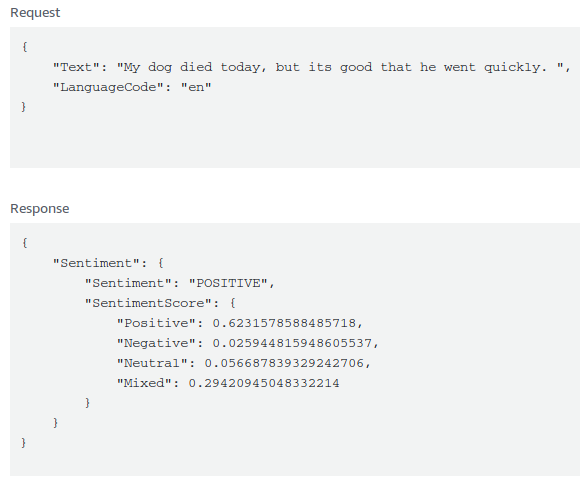
\includegraphics[scale=0.5]{./LitReview/images/comphrendResult.png}
\label{aws:sentiment}
\end{figure}

Getting confused with sentences that are actually negative, but include words like 'happy' is common issue with existing sentiment tools and one that should be solved by not only analysing the valence of a text, but looking at the text in more ways than just the positivity of it and taking into account the whole sentence.

\subsection{Sentiment Analysis Research}

There seems to be very little existing work which tries to use semantic analysis to predict more than just the valence of text, as most existing work is only considering how positive or negative the input is. Attempting to predict a more descriptive form of the emotion of the input will be a challenge.

When analysing the positivity and negativity of tweets, using a lexicon based approach as well as machine learning approaches have been used \cite{kolchyna2015twitter} \cite{go2009twitter} to great effect. In this case, a combination of the two has proved to be the most effective. Investigating whether these approaches work just as well when taking into account more than just the valence of the text will be the majority of the work on this project.

Existing sentiment analysis research processes the data a large amount before any machine learning is done on it, for example by removing all the words which lie exactly in the middle of the valence scale.  \cite{kolchyna2015twitter} The different pre-processing methods will also be compared during this project.

\subsection{Spotify}
With Spotify API being very easy to access for developers, there already exists large numbers of web applications that utilise the data that Spotify provides. Creating a basic web app with HTML front and a Node.js back end is very straightforward \cite{spotifyHello}, with extensive documentation being provided by Spotify, and there are many other online sources to facilitate the building of this part of the application. 

A project which is similar to the Spotify API that will be created as part of the web application that will showcase the output of the sentiment analysis tool is the MoodTape web app, which generates playlists using the users top artists and a valence value between 0 and 1 \cite{moodtape}.
In the production of this application, it was discovered that some songs which would be described as 'popular party songs' are valued with low valence scores due to having a large amount of minor chords. To deal with this, they incorporated the energy and danceability attributes. 
This application only takes in values from 0 to 1 as a mood, and an improvement that could be made is to try and move away from inputting numeric values to inputting a mood. The use of creating the playlist based on the users top artists is something that was not considered before, and now will be factored into future production plans.

The Spotify solution to be created will be a RESTful API built with Node.js, which has already been prototyped and will be easy to continue work on, due the the amount of documentation available \cite{spotifyHello}.

\begin{lstlisting}[style=leftCode, caption={Some of the attributes of a song obtained through requesting information through the Spotify API},captionpos=b, label={spotifyJSON}]
{
    "danceability": 0.322,
    "energy": 0.0593,
    "key": 1,
    "loudness": -53.057,
    "speechiness": 0.0444,
    "acousticness": 0.908,
    "instrumentalness": 0.708,
    "liveness": 0.121,
    "valence": 0.0165,
    "tempo": 158.402,
    "time_signature": 4
}
\end{lstlisting}

\section{Sentiment Representation Structures}
\subsection{Ekman's Six Basic Emotions}

There is no universally accepted model for representing emotion, but a standard for classifying emotions in a categorical model is using Ekmans six basic emotions \cite{Ekman}. These are identified as Anger, Disgust, Fear, Happiness, Sadness and Surprise. Being able to use these fundamental emotions to represent the sentiment of a text allows for more insight into the emotions around it. Since there are only six discrete classes in which emotions can be placed, this can be argued to be very subjective when classifying however \cite{emoBank}.

\subsection{Valence}
A very common way to classify phrases and sentences in sentiment analysis is to analyse the valence of the text \cite{frijda1986emotions}.

The valence of a piece of text is how positive or negative the emotion behind it is. An example of a sentence with a high valence would be "I am feeling very happy, I'm having a great day!", compared to a low valence, "I am having a terrible day, everything is going wrong". 

As this is a dimensional model, where values chosen could be hypothetically infinite this can represent a wider range than just six classes such as Ekmans emotions, however only measuring the positivity or negativity of a text does not provide much insight into it.
Using valence in a machine learning context is very useful though, as commonly the valence values can be put into discrete binary classes, positive or negative, and is a good base to start from.

\subsection{Circumplex Model}
The Circumplex Model is a 2 dimensional way of representing emotions, using a Valence or Pleasure measure and an Arousal or Activation measure \cite{modelOfAffect}.

\begin{figure}[h]
\caption{Graph of the Circumplex model with the $x$ axis representing the Valence and the $y$ axis representing the Arousal}
\centering
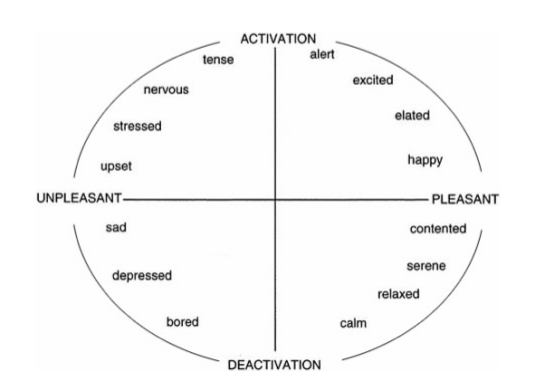
\includegraphics[scale=0.4]{./LitReview/images/circumplex.png}
\end{figure}

However there have been issues raised with this model \cite{circumplexIssues},  with concerns that only having two dimensions is not enough to be able to properly classify a human emotion.

\subsection{Valence Arousal Dominance Structure}
Building on the Circumplex Model, combating some of the issues raised with it comes the Valence-Arousal-Dominance Structure.
Known also as the as the Pleasure-Arousal-Dominance, the Valence-Arousal-Dominance structure (referred hereafter as VAD) introduced in 1974 \cite{PAD} \cite{VAD} provides a 3D representation for emotions, with each variable being defined as follows:
\begin{itemize}
    \item Valence- How positive or negative the statement is.
    \item Arousal- Degree of calmness or excitement, the energy of the statement. 
    \item Dominance- Degree of control over a situation.
\end{itemize}

Using VAD values allow for easy representation into the Ekman six basic emotions, as although there is no standard on the exact VAD values to use for each emotion, the primary dataset that will be used references values given by Russell and Mehrabian \cite{VADMapping}, which are shown below:

\begin{center}
\begin{tabular}{ |c|c|c|c|c|c|c| } 
 \hline
  & Anger & Disgust & Fear & Happiness & Sadness & Surprise \\ 
 \hline                        
 Valence & -0.51 & -0.6 & -0.64 & 0.81 & -0.63 & 0.4\\ 
 Arousal & 0.59 & 0.35 & 0.6 & 0.51 & -0.27 & 0.67\\ 
 Dominance & 0.25 & 0.11 & -0.43 & 0.46 & -0.33 & -0.13\\ 
 \hline
\end{tabular}
\end{center}

\begin{figure}[h]
\caption{Graph showing the affective space spanned by the three VAD dimensions showing Ekmans six basic emotions \cite{VADMapping}}
\centering
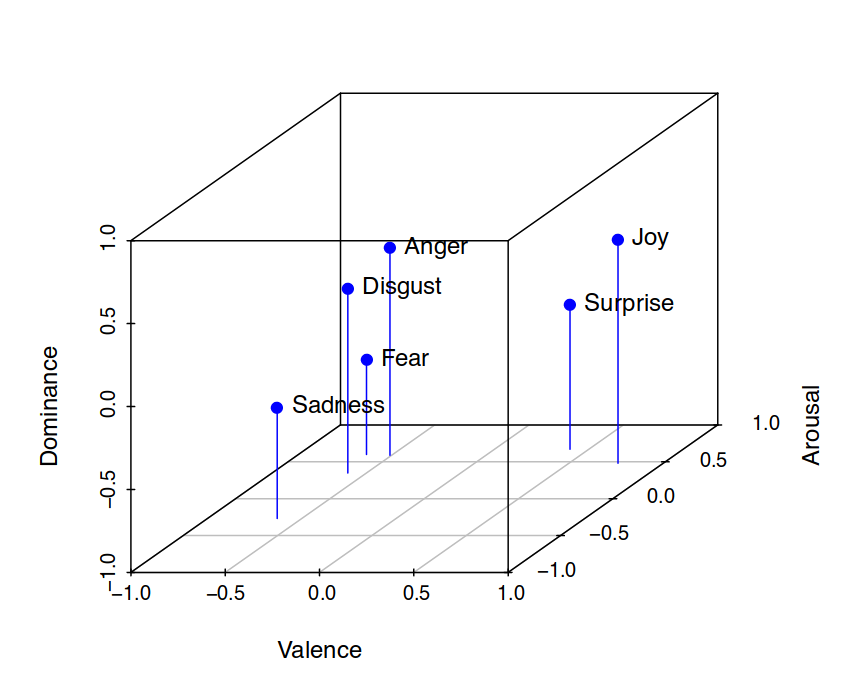
\includegraphics[scale=0.2]{./LitReview/images/VAD_Ekman.png}
\label{ekmans:graph}
\end{figure}

Using the VAD structure to represent sentiment in this project was ideal, as it allows for much more description of emotion in text \cite{emotionPerspective}, and having numeric values means its easy to work with.

\section{Available Data}
There are two suitable datasets for this task, which will both be used to train the sentiment analysis tool on.
\subsection{EmoBank}
This dataset is the most important one for this project, as it contains 10,000 English sentences covering multiple genres, all annotated with their own VAD values \cite{emoBank}.

\begin{center}
\begin{tabular}{ |c|c| } 
 \hline
  Sentence Type & Frequency \\ 
 \hline         
 News Headlines & 1192 \\
 Blogs & 1336 \\
 Essays & 1135 \\
 Fiction & 2753 \\
 Letters & 1413 \\
Newspapers & 1314 \\
 Travel Guides & 919\\
 \hline
 Sum & 10062 \\
 \hline
\end{tabular}
\end{center}

This dataset contains VAD values for each piece of text from both writer and the reader of the text, but due to the findings in \cite{emoBank} only the values given by the reader will be used, as it is concluded that this perspective has higher emotionality and therefore they should be easier to train with.

Initial prototyping using this dataset shows that it is easy to implement into machine learning tools, but there is an issue with the distribution of data, as shown in Figure \ref{emoBank:dist}. When the sentences are split into buckets depending on their valence values, there is a very large disparity in the frequency of each bucket represented, meaning that training on this dataset leads to incorrect classification of test data.

\begin{figure}[h]
\caption{Graph showing the distribution of the valence of all the sentences in the EmoBank corpus, with 0 being very negative and 10 being very positive}
\centering
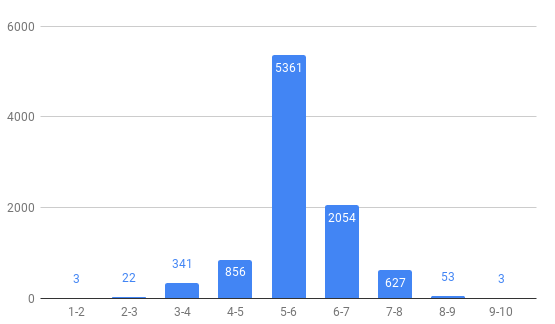
\includegraphics[scale=1.8]{./LitReview/images/valence-frequency-bucket-graph.png}
\label{emoBank:dist}
\end{figure}

Another issue with this dataset is that because it is not big enough, it is occasionally incorrectly classifying words as negative which shouldn't be. An example of this is where it repeatedly classifies "Italy" as being a negative word. This is due to the dataset containing a letter from someone who had an unpleasant holiday in Italy. To counteract this issue, I plan on using more data in conjunction with this dataset so hopefully this situation will become less prevalent.

So far in prototyping the sentiment analysis tool on this has only been trying to predict the valence of the words. Trying other classification systems has not been done yet, and is currently in production. 

\pagebreak

\subsection{Affective Ratings for Words}
To increase the range of data to train with, a dataset that contains VAD values for almost 14,000 English words\cite{wordsData} is also being incorporated, and can help balance out unnecessarily strongly weighted words by reclassifying them into a more appropriate emotional state. The issue with having only the individual words rated with VAD values means that the context in which the words are used can be lost, so this is a case where using a bag-of-words method for splitting up the sentences may not be the most appropriate.

\begin{figure}[h]
\caption{Graph showing the distribution of the valence of all the sentences in the EmoBank corpus, with 0 being very negative and 10 being very positive}
\centering
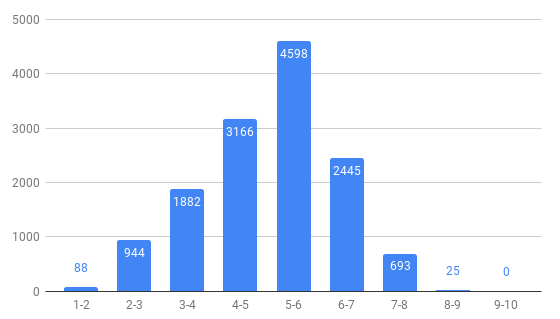
\includegraphics[scale=1.9]{./LitReview/images/words-valence-buckets.png}
\label{words:dist}
\end{figure}

\section{Data Pre-Processing}

\subsection{Tokenisiation}

Splitting the words up using a 'Bag of Words' method, where the order of the words does not matter, just the frequency of the words within the sentence.

By not taking any training into account and just

The disadvantage of this method is that it loses some of the context in which the words are written in. An example is the sentence "They were not happy". Taking each word individually, this can cause mis-evaluation, and a way to improve this is to use N-Grams to tokenise the words. 

N-Grams in a text analysis approach will be to take the set of words, so that the spatial awareness within the sentence can be taken into account. For example when the above example sentence is put into a bigram model, the tokens are as follows:

\begin{center}
"They were" \\
"were not"\\
"not happy"\\
\end{center}

Here we can see the 'not' will be taken into account, negating the sentiment of the "happy", giving a better understanding of the true sentiment.

A varying value for N will be trialled as part of the project.

\subsection{Stemming and Lemmatization}

Stemming and Lemmatizing words reduces words down to their base, for example the word "Approaching" can be reduced down to the word "Approach". The sentiment behind the word will stay the same, it just removes the affixes, allowing for easier processing. This will be done by using one of the many integrated NLTK lemmatizing libraries \cite{lemmatizing}

\subsection{Handling Negation}

The use of the word "not" before a strongly valued word needs to be taken into account as can change the whole sentiment of a sentence. 
What has been used before to great effect was to reverse the sentiment score of every word appearing between a negation and a punctuation mark (.,!?:;) \cite{kolchyna2015twitter}. 

\subsection{Stop Words}

Stop words are words which carry a connecting function in the sentence, such as prepositions and have no true influence on the emotions behind the sentence. Research has been done on the best way to remove these irrelevant words \cite{saif2014stopwords}, and it has been found that removing the most common irrelevant words compiled in a list, words such as "don't" or "and", causes classification algorithms to decrease in accuracy. Exploring this further will be a stretch goal for the project, since there are suggestions that small changes, such as removing words that only occur once in a body of text help improve prediction accuracy. 
\section{Emotion Classification}

Processing the data into a format which is most beneficial to analyse important, and how the data is classified is an issue which requires research.

Since the variables for Valence, Dominance and Arousal are all continuous, classifying them into discrete classes is ideal and there are primarily three ways that are being considered.

\subsection{Ekmans Emotions}
One option is for each item in my combined training corpus is to combine the VAD values and assign the text a computed Ekman Basic Emotion\cite{Ekman}. 
This has the advantages letting the data be classified into six discrete classes which should allow easier classification of training data, but has the disadvantages of only giving six possible emotions, which does not help as the goal is to provide a greater insight into the sentiment of the text and limiting this to only six options is restrictive.

\subsection{Bucketing Variables}
Another option is splitting the values for each dimension up into buckets, and running a prediction for each value for the target sentence. 
This is what has been used for prototyping so far, and this has proven to be wildly inaccurate since the distributions for the variables are so unevenly weighted over the dataset.

\subsection{More Emotion classes}
In Russell's 1977 paper \cite{VADMapping} that the earlier values for Ekman's six basic emotions in Figure \ref{ekmans:graph} were obtained, there are also the VAD values for 145 other emotions such as 'Excited' (VAD: 0.62,0.75,0.25). Using the most useful of these emotions could lead to greater understanding of the data, and would lead to more insightful analysis into the input text. Splitting the data into 145 distinct classes is definitely a step too far, but a balance can be found with the ideal number of them, which can be trialled as part of the project if there is time (but this is not a priority).

Each sentence will be classified based on which emotion it is closest to on a 3D graph, using the shortest distance between points.
\section{Analysis Approaches}

There are two fundamental ways of analysis sentiment from a piece of text, each with their own advantages and disadvantages. Both will be explored during this project.

The evaluation metric to compare the analysis approaches will be to compare the  Mean Absolute Percentage Error, calculated by the following: 

$$ MAPE = \frac{100\%}{n} \sum_{t=1}^{n} \left| \frac{A_t-F_t}{A_t} \right| $$
where $A_t$ is the actual value and $F_t$ is the predicted value.

\subsection{Lexicon-Based}

By taking the words in a Bag of Words and N-Gram format, a VAD value will be assigned to each word, or set of words and an overall score can be calculated for the sentence by totalling up average score for the sentence. This is a basic place to start from, and provides good results to compare the Machine Learning accuracy predictions to. 

\subsection{Machine Learning}

In multiple cases using a Naive Bayes Classifier and using Support Vector Machines showed the best results in previous semantic analysis research \cite{kolchyna2015twitter} \cite{go2009twitter}, so these will be a priority for analysing effectiveness however more can be taken into account if there is time.

Using Python is a clear choice for developing the Sentiment Analysis tool, due to the prevalence of Natural Language Processing (NLP) and Machine Learning libraries and the documentation in these areas is good. I will primarily make use of the NLTK library \cite{NLTKBook}, which contains features for NLP and basic Machine Learning on sentences and words. 



\section{Text entry method}

In the proposal for this project, it was suggested that an interesting way of getting the input text from the user would be to implement a chatbot interface within a web app, using a plugin service to facilitate this. 

There are many platforms available on which chat bots can be built like Slack or WhatsApp, but the decision has been made to look more into Facebook and Microsoft's solutions since these are the ones with the largest amount of documentation.

\subsection{Facebook Bot Platform}

The platform itself offers some basic Natural Language Processing, but primarily the platform is aimed at businesses, below is the entities in input text that the inbuilt NLP can pick up on and separate out:

\begin{center}
\begin{tabular}{ |c| } 
 \hline
  Recognised Categories \\ 
 \hline                        
 Greeting \\
 Thanks \\
 Bye \\
 Date/Time \\
 Amount of Money \\
 Phone numbers \\
 Email address \\
 Distance \\
 Quantity \\
 Temperature \\
 Volume \\
 Location \\
 Duration \\
 URL \\
 Sentiment \\
 \hline
\end{tabular}
\end{center}

The only category that would be used is the sentiment recognition, but during prototyping this could not be made to work, and there seems to be very few examples of projects using this tool.
Since building the sentiment analysis tool is part of this project, the bot platform not offering useful NLP is not disastrous. 
Issues with this platform include limited access to testing tools while developing, until the bot is approved by Facebook itself which can take a long time, so this may not be the best platform to use. 

\subsection{Microsoft Bot Framework using Azure}

Microsoft's Bot Framework can be implemented through Skype \cite{Azure}, and can be linked up with the Microsoft Language Understanding system, LUIS \cite{LUIS}. This system primarily is built for businesses, and attempts to get the input text intent and entities, as shown below.
\begin{center}
\begin{tabular}{ |c|c|c| } 
 \hline
  User Input & Intent & Entities \\ 
 \hline                        
 Book a flight to Seattle & BookFlight & Seattle \\
 When does your store open? & StoreHoursAndLocation & open \\
 Schedule a meeting at 1PM with Bob in Distribution & ScheduleMeeting & 1PM, Bob \\
 \hline
\end{tabular}
\end{center}

This does not have any inbuilt sentiment analysis which isn't an issue since this is being built separately, but prototyping with this framework and using it for past projects has been difficult to set up, and has been slow.

\subsection{An Alternative}

When the use of a chatbot was suggested during the project proposal, there were issues with this idea raised to do with validating the Spotify account through a chat system. 
After more research into the abilities of the chatbot platforms and how the Spotify Authorisation API works, an alternative would be is to not use a chatbot platform at all for user text input.
There appears to be no available way to allow users to log into their Spotify Account through a messaging system, and as shown in Figure \ref{spotify:auth}, the tokens would have to be generated through a web app on a page, and then having to pass it through the third party bot platform is much more work and seems like unnecessary effort. 

\begin{figure}[ht]
\caption{Diagram from the Spotify Documentation showing the authorisation flow for using the Spotify API \cite{spotifyHello}}
\centering
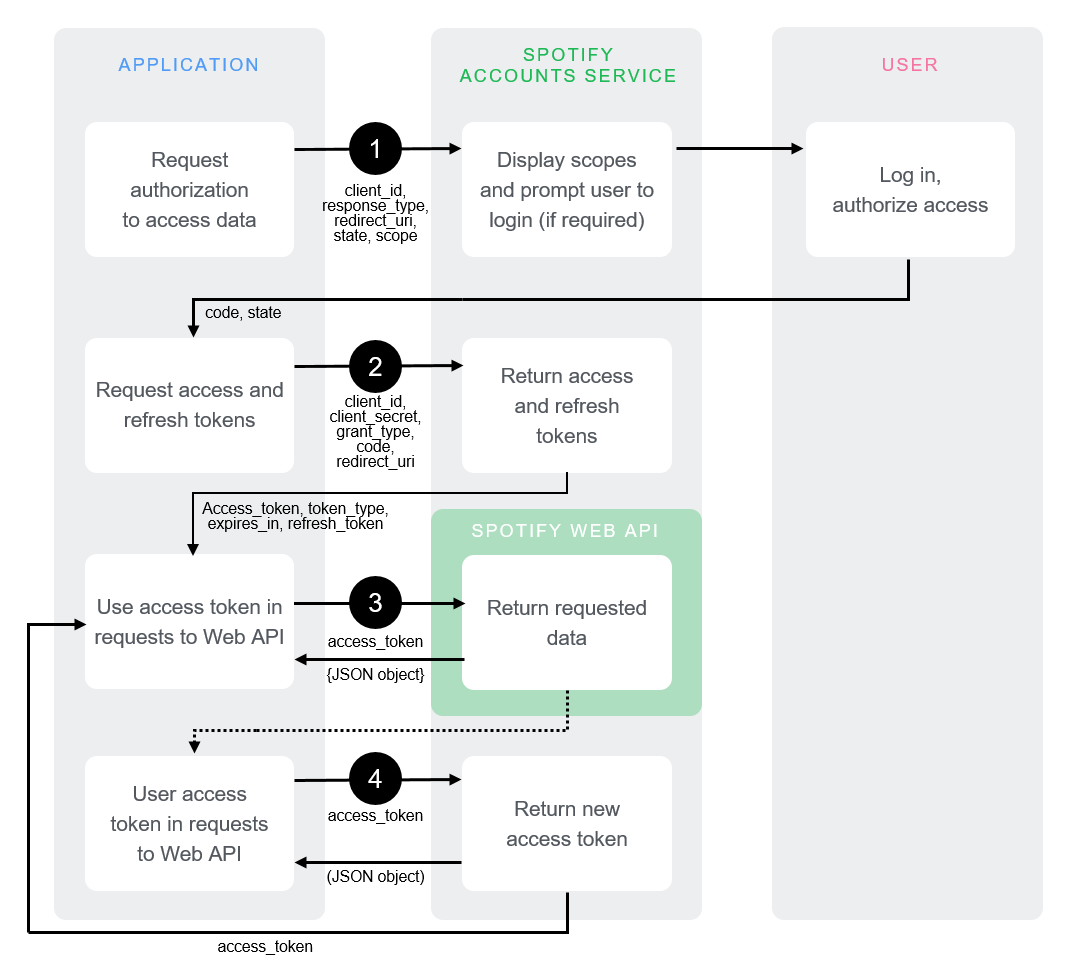
\includegraphics[scale=0.3]{./LitReview/images/spotifyAuthGuide.png}
\label{spotify:auth}
\end{figure}

An alternative would be to have a web application with a forms interface, allowing text box entry. This would still serve exactly the same purpose with easier implementation from a development point of view, since there will be no going through a third party. 
The prompts for emotive user input text can still change and be relevant as logic can be implemented within the web application on the front end with JavaScript. 

After this research into the chatbot platforms, the conclusion has been made that using this method for data input is unnecessarily complex, doesn't add much and would cause issues for the more important part of the project, which is the Spotify API integration. As shown in Figure \ref{programFlow}, the project will be restructured, with the text being input through the use of a forms system on the web application.

\begin{figure}[h]
\caption{The new structure of the project}
\centering
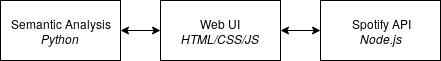
\includegraphics[scale=0.5]{./LitReview/images/ProgramFlow.png}
\label{programFlow}
\end{figure}


\section{Conclusion}
Due to the research done, there is now a clearer plan for moving forward with this project. Unnecessary parts have been removed, and there is a more specific focus for how the sentiment analysis tool is going to work. 
There is extra time to work on the machine learning side of the project, meaning there is now the opportunity for more experimentation with different methods.

Decisions still need to be made, such as the exact emotion classes from the Emotional Classification Table given by Russell \cite{VADMapping}, but progress is happening and there is a plan of how to move forward from this point.